\section{Address Generator}

Students used two~74LS590 8-bit counters to generate the sixteen
least-significant bits of the address generator, as instructed by the lab
manual.  By wiring the most significant bit of one IC into the clock of the
second IC, the two counters will respectively produce the lower byte and higher
byte of the aforementioned sixteen bits.  A similar technique was used to
generate the most significant bit.  By using bit 15 (zero-indexed) as the clock
for a JK flip-flop, bit 16 of the address generator was produced with an
accurate timing.  Figure~\ref{f:add_gen} shows bits 15 and 16 functioning
properly.
%
\begin{figure}[H]
\centering
	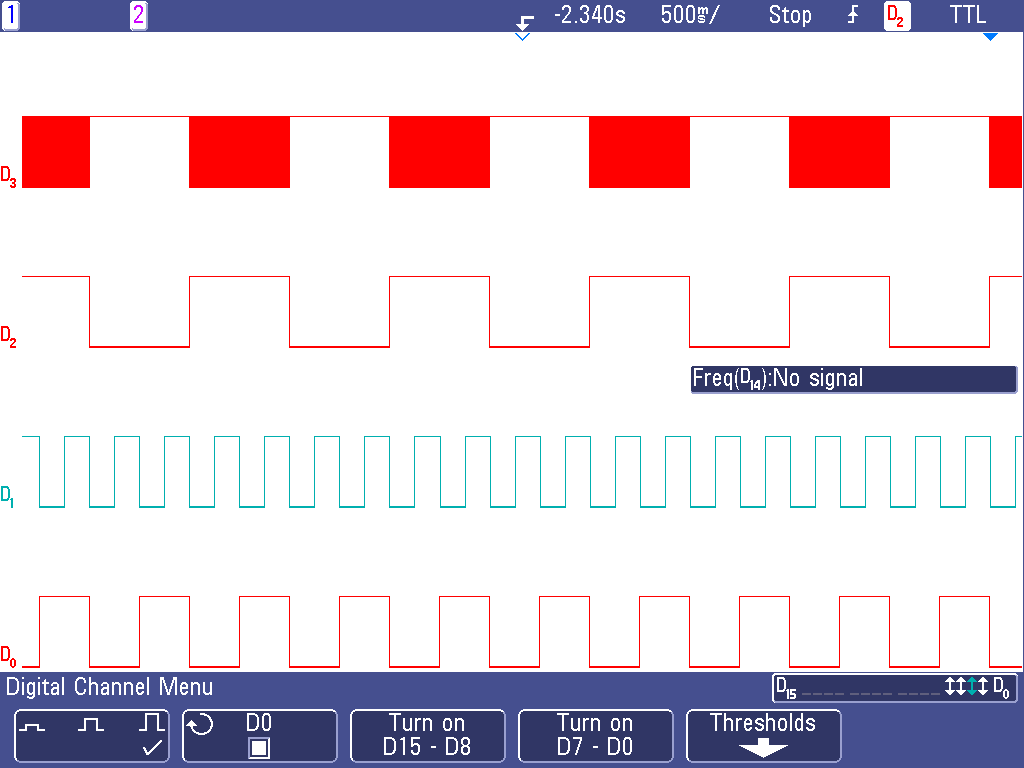
\includegraphics[width=.8\textwidth]{img/shot/add_gen.png}
	\parbox{.8\textwidth}{
	\caption[Functioning Address Generator]{Oscilloscope screenshot of the
	functioning address generator. Note that \ttt{D1} and \ttt{D0} represent
	zero-indexed bits 15 and 16.  Note also that \ttt{D2} and \ttt{D3}
	represent the \ttt{OE} and \ttt{WE} pins.}
	\label{f:add_gen}}
\end{figure}
